\chapter{Análisis de datos ingestados en el lago de datos}

En este apartado, se busca realizar una serie de consultas analíticas para demostrar al cliente cómo poder extraer información relevante para su caso de uso. Además, también se busca demostrar cómo persistir datos agregados en una nueva tabla para poder ser consultados de manera más rápida por herramientas de BI o de Dashboarding.

\section{Consultas}

\subsection{Preparación de las consultas}

Para poder ejecutar las consultas vamos a cargar los dataframes que hemos guardado en el lago de datos:

\begin{lstlisting}[language=scala]
import java.util.Properties
val properties = new Properties()

properties.setProperty("user", "postgres")
properties.setProperty("driver", "org.postgresql.Driver")
properties.setProperty("password", "postgres")
properties.setProperty("partitionColumn", "altitude")
properties.setProperty("lowerBound", "0")
properties.setProperty("upperBound", "2000")
properties.setProperty("numPartitions", "10")
properties.setProperty("password", "postgres")

val df_airports = spark.read.option("partitionColumn", "altitude").option("lowerBound", 0).option("upperBound", 2000).option("numPartitions", 10).jdbc("jdbc:postgresql://localhost:5432/postgres", "airports", properties)

val df_airlines = spark.read.format("parquet").load("hdfs://localhost:9000/practica/airlines/")
val df_countries = spark.read.format("csv").option("header", "true").option("inferSchema", "true").load("hdfs://localhost:9000/practica/countries/")

val df_routes=spark.read.format("org.apache.spark.sql.cassandra").option("spark.cassandra.connection.host","127.0.0.1").option("spark.cassandra.connection.port","9042").option("keyspace", "practica").option("table", "routes").load()
\end{lstlisting}

Ahora pasaremos los dataframes a \texttt{TempViews} para poder realizar consultas SQL sobre ellos:

\begin{lstlisting}[language=scala]
df_airports.createOrReplaceTempView("airports")
df_airlines.createOrReplaceTempView("airlines")
df_countries.createOrReplaceTempView("countries")
df_routes.createOrReplaceTempView("routes")
\end{lstlisting}

\begin{figure}[H]
    \centering
    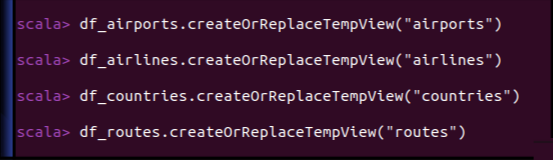
\includegraphics[width=0.8\textwidth]{figures/59.png}
    \caption{Creación de las vistas temporales de los dataframes}
    \label{fig:tempviews}
\end{figure}

\subsection{¿Qué aeropuerto está a mayor altitud (columna altitude)?}

La primera consulta que se nos pide es obtener los aeropuertos con mayor altitud. Para ello, se ha realizado la siguiente consulta:

\begin{lstlisting}[language=scala]
spark.sql("SELECT * FROM airports ORDER BY altitude DESC LIMIT 1").show()
\end{lstlisting}

\begin{figure}[H]
    \centering
    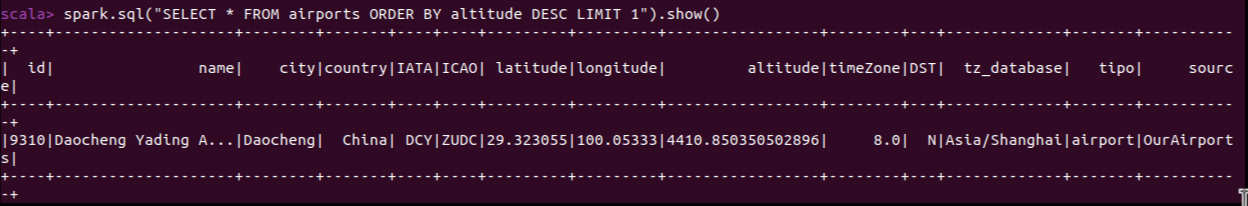
\includegraphics[width=0.8\textwidth]{figures/60.png}
    \caption{Resultado de la consulta de aeropuertos con mayor altitud}
    \label{fig:consulta1}
\end{figure}

\subsection{¿Cuántos aeropuertos hay en España (Spain)?}

La segunda consulta que se nos pide es obtener el número de aeropuertos que hay en España. Para ello, se ha realizado la siguiente consulta:

\begin{lstlisting}[language=scala]
spark.sql("SELECT COUNT(country) AS airports_total FROM airports WHERE country == 'Spain'").show()
\end{lstlisting}
